\documentclass[12pt,a4paper]{article} 

\usepackage[russian]{babel}
\usepackage[T2A]{fontenc} 
\usepackage[utf8]{inputenc} 
\usepackage{graphicx}
\usepackage{amsmath}
\usepackage{amssymb}
\usepackage{amsfonts}
\usepackage{geometry}

\geometry{a4paper, total = {170mm, 257mm}, left = 20mm, top = 20mm}
\frenchspacing 

\renewcommand{\baselinestretch}{1.3}

% counter
\newcounter{problem}
\renewcommand{\theproblem}{\arabic{problem}.}
\newcommand{\problem}{\refstepcounter{problem}\textbf{Задача~\theproblem~}}

% convenient commands
\newcommand{\boldVec}[1]{\vec{\mathbf #1}}
\newcommand{\vectorProduct}[2]{\boldVec #1 \times \boldVec #2}
\newcommand{\scalarProduct}[2]{(\boldVec #1, \boldVec #2)}

\begin{document}
    \begin{center}
        {\textbf 
            {\Large
                Дифференциальная геометрия
                \\
                Домашнее задание №1
                \\
                <<Кривые и поверхности в пространстве>>
                \\
                ФН2-42Б, 2 курс, 4 семестр
                \\
                Арсений Токарев, Вариант 2-23
                \\
            }
        }
    \end{center}

    \section*{Дано: }

    \hspace{5mm} Поверхность задана параметрически уравнениями $ S \colon \boldVec r = \boldVec r(u, v), \  u, v \in \mathbb{R} $.

    Уравнение поверхности: 
    \[ \boldVec r(u, v) = \{ \cosh u \cos v,\ 5 \sinh u,\ \cosh u \sin v \}. \]

    Вид кривой на поверхности и координаты точек: 
    \[ \gamma \colon u = v,\ P_1(1, 0, 0),\ P_2(-\cosh \pi, 5 \sinh \pi, 0). \]

    \section*{Задачи: }


    \hspace{7mm}\problem Найти особые точки параметризированной поверхности. Составить уравнение касательной к поверхности в точках $ P_1 $ и $ P_2 $.
    
    \bigskip

    Для того, чтобы вывести уравнение касательной плоскости к поверхности в точке, необходимо найти вектор к поверхности в данной точке. Сначала нужно взять частные производные $ \frac{\partial \boldVec r}{\partial u} = \boldVec r_u $ и $ \frac{\partial \boldVec r}{\partial v} = \boldVec r_v \colon$
    \[
        \boldVec r_u = 
            \begin{pmatrix}
                \sinh u \cos v
                \\
                5\cosh u
                \\
                \sinh u \sin v
            \end{pmatrix}\! , \  
        \boldVec r_v = 
            \begin{pmatrix}
                -\cosh u \sin v
                \\
                0
                \\
                \cosh u \cos v
            \end{pmatrix}\! ,
    \]

    \noindent затем векторно их перемножить:
    \[
        \vectorProduct{r _u}{r_v} = 
            \begin{vmatrix}
                i && j && k
                \\
                \sinh u \cos v && 5\cosh u && \sinh u \sin v
                \\
                -\cosh u \sin v && 0 && \cosh u \cos v
            \end{vmatrix}
        =
    \]

    \noindent $ = \boldVec i\,(5 \cosh^2 u \cos u ) + \boldVec j\,(\sinh u \cosh u \cos^2 - \sinh u \cosh u \sin^2 v) + \boldVec k\,(5 \cosh^2 u \sin v) $
    \[
       \vectorProduct{r_u}{r_v} =
        \begin{pmatrix}
            5 \cosh^2 u \cos v
            \\
            -\sinh u \cosh u
            \\
            5 \cosh^2 u \sin v
        \end{pmatrix}\! .
    \]

    Сразу можно заметить, что $ \boldVec r_u \times \boldVec r_v \ne \vec{\textbf 0}$ ни при каких значениях $ u \ \text{или} \ v $. Это означает, что все точки поверхности -- регулярные.

    Посчитаем норму векторного призведения $ | \boldVec r_u \times \boldVec r_v | \colon$ 
    \[
        | \boldVec r_u \times \boldVec r_v | = \sqrt{25 \cosh^4 u + \sinh^2 y \cosh^2 u} = \cosh u \sqrt { 25 \cosh^2 u + \sinh^2 u }\, . 
    \]

    Таким образом, вектор нормали $ \vec{\textbf n} $ имеет следующий вид: 
    \[
        \vec{\textbf n} = \frac{\boldVec r_u \times \boldVec r_v}{| \boldVec r_u \times \boldVec r_v |} = \frac{1}{\sqrt{25 \cosh^2 u + \sinh^2 u}}
        \begin{pmatrix}
            5 \cosh u \cos v
            \\
            -\sinh u
            \\
            5 \cosh u \sin v
        \end{pmatrix} \! .
    \]

    Выразим координаты точек $ P_1 $ и $ P_2 $ через $ u \ \text{и} \ v $. Для этого приравняем координаты уравнения поверхности $ \boldVec r(u, v) $ к координатам этих точек:
    \begin{table}[h]
        \centering
        \begin{tabular}{lcl}
            $
                P_1 \colon
                \begin{cases}
                    \cosh u \cos v = 1,
                    \\
                    5 \sinh u = 0,
                    \\
                    \cosh u \sin v = 0.
                \end{cases} 
            $ 
            & $ \Leftrightarrow $ & 
            $
                \begin{cases}
                    u_1 = 0,
                    \\
                    v_1 = 0.
                \end{cases}
            $

            \\ \\

            $
                P_2 \colon
                \begin{cases}
                    \cosh u \cos v = -\cosh \pi,
                    \\
                    5 \sinh u =  5 \sinh \pi,
                    \\
                    \cosh u \sin v = 0.
                \end{cases}
            $ 
            & $ \Leftrightarrow $ & 
            $
                \begin{cases}
                    u_2 = \pi,
                    \\
                    v_2 = \pi.
                \end{cases}
            $

        \end{tabular}
    \end{table}

    Теперь можно найти нормали касательных плоскостей в точках $ P_1 $ и $ P_2 $ соответсвенно. В точке $ {P_1} $ вектор единичной нормали равен:
    \[
        \vec{\textbf n}|_{P_1} =
        \begin{pmatrix}
            1 
            \\ 
            0 
            \\ 
            0  
        \end{pmatrix}\! ,
    \]

    \noindent тогда касательная плоскость имеет вид: 
    \[
        T|_{P_1} \colon x - 1 = 0.
    \]


    В точке $ {P_2} $ вектор единичной нормали равен:
    \[
        \vec{\textbf n}|_{P_2} = \frac{1}{\sqrt{25 \cosh^2 \pi + \sinh^2 \pi}}
        \begin{pmatrix}
            -5 \cosh \pi
            \\
            -\sinh \pi
            \\
            0
        \end{pmatrix}\! , 
    \]

    \pagebreak

    \noindent и касательная плоскость имеет вид: 
    \[
        T|_{P_2} \colon 5 \cosh \pi \cdot x + \sinh \pi \cdot y + 5 = 0.
    \]

    \bigskip

    \begin{flushright}
        \begin{tabular}{rl}
            \textbf{Ответ:} & Особых точек нет,

            \\

                            & $ T|_{P_1} \colon x - 1 = 0 $,

            \\

                            & $ T|_{P_2} \colon 5 \cosh \pi \cdot x + \sinh \pi \cdot y + 5 = 0 $.
        \end{tabular}
    \end{flushright}

    \bigskip

    \problem Исследовать зависимость вида поверхности от области изменения параметров $ (u, v) $. Составить уравнения координатных линий. Построить поверхность и координатную сеть на ней (с использованием системы компьютерной алгебры Wolfram Mathematica)

    \bigskip
    
    Уравнение поверхности, выраженное через $ x, y, z \colon$
    \[
        \begin{cases}
            x = \cosh u \cos v,
            \\
            y = 5 \sinh u,
            \\
            z = \cosh u \sin v,
        \end{cases} 
        \Leftrightarrow \ 
        x^2 + z^2 - \frac{y^2}{25} = 1, 
    \]

    \noindent значит, данная поверхность -- однополостный гиперболоид с осью вдоль $ OY $ (рис. \ref{fig:hyp}).

    \begin{figure}[!h]
        \centering
        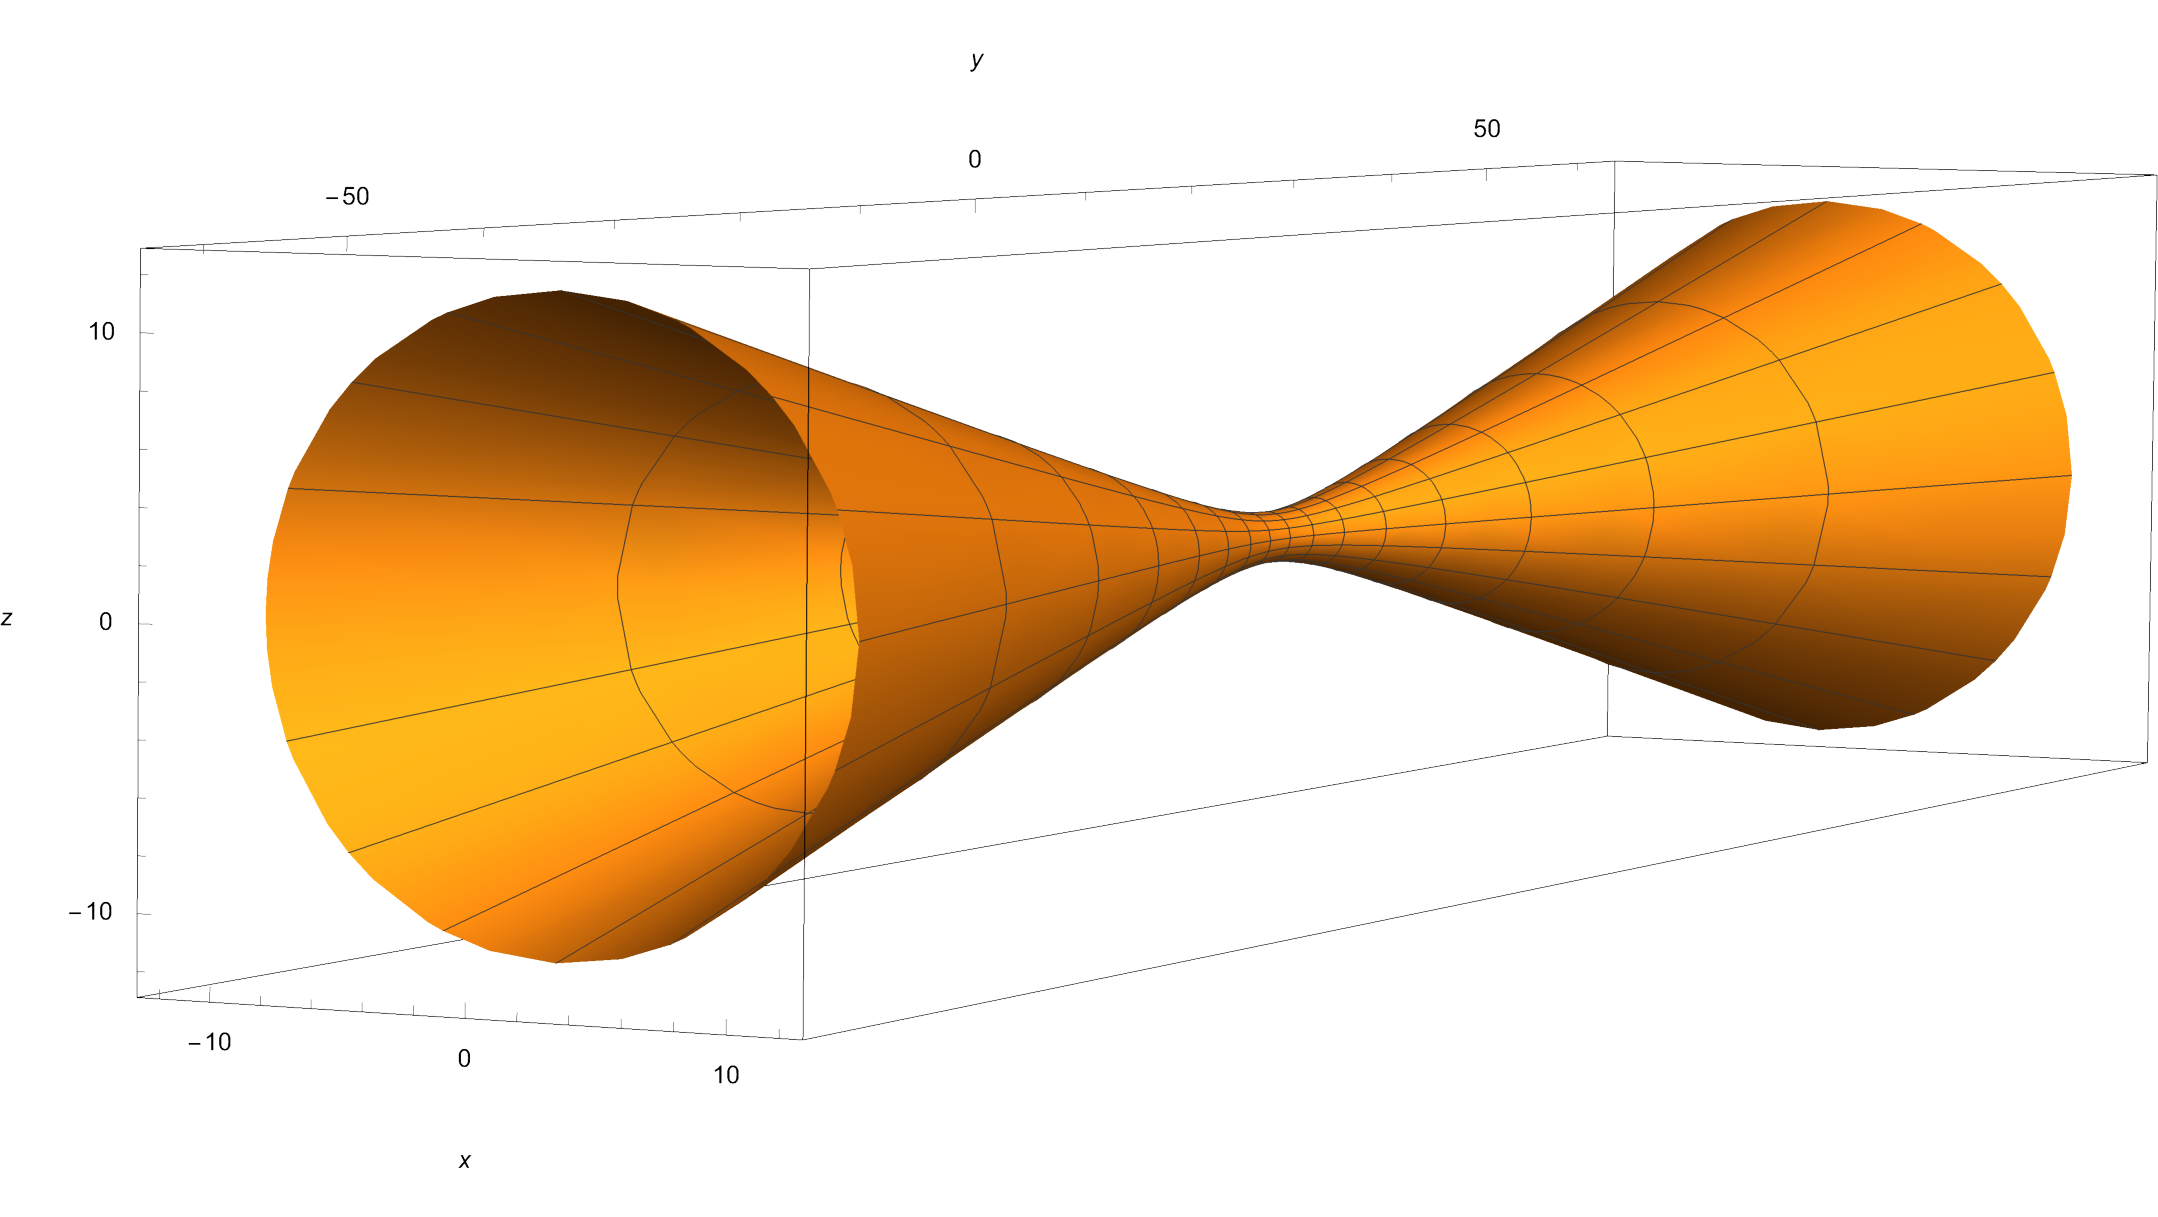
\includegraphics[width=0.8\textwidth]{Hyp.pdf}
        \caption{Однополостный гиперболоид}
        \label{fig:hyp}
    \end{figure}

    Рассмотрим координатные линии данной поверхности. При $ u_0 = const $ получаем:
    \[
        x^2 + z^2 = const,\, const = R = \sqrt{1 + \frac{y^2}{25}} = \cosh u_0,
    \]

    \noindent то есть уравнения окружностей с радиусами $R = \cosh u_0$. А при $v_0 = const$ получаем се\-мейство гипербол.

    \begin{flushright}
        \begin{tabular}{rl}
            \textbf{Ответ:} & Однополостный гиперболоид,

            \\

                            & $ (u_0, v) $ -- окружности,

            \\

                            & $ (u, v_0) $ -- гиперболы.
        \end{tabular}
    \end{flushright}

    \pagebreak

    \problem Вычислить первую квадратичную форму поверхности. Вычислить угол между кривыми $ l_1 \colon u = v^2 $ и $ l_2 \colon u = v $ в точке их пересечения.

    \bigskip

    Вычислим коэффициенты первой квадратичной формы:
    \[
        \begin{tabular}{l}
            $ E(u,v) = \scalarProduct{r_u}{r_u} = \sinh^2 u + 25 \cosh^2 u $,
            \\ \\
            $ M(u,v) = \scalarProduct{r_u}{r_v} = 0 $,
            \\ \\
            $ G(u,v) = \scalarProduct{r_v}{r_v} = \cosh^2 u $,
        \end{tabular}
    \]
    
    \noindent значит, матрица первой квадратичной формы имеет вид: 
    \[
       \mathbb{G}(u, v) = 
       \begin{pmatrix}
           \sinh^2 u + 25 \cosh^2 u & 0
           \\
           0                        & \cosh^2 u
       \end{pmatrix}\! .
    \]

    Угол между кривыми -- это угол между векторами их скоростей в точке их пересечения. Его можно вычислить по следующей формуле:
    \[
        \cos \alpha = \frac {
            (\boldVec \xi_1)^T \cdot \mathbb{G} \cdot \boldVec \xi_2
        } {
            \sqrt{(\boldVec \xi_1)^T \cdot \mathbb{G} \cdot \boldVec \xi_1}
             \cdot 
             \sqrt{(\boldVec \xi_2)^T \cdot \mathbb{G} \cdot \boldVec \xi_2}
        }
    \]
    
    Для нахождения точек пересечения и для вычисления векторов скоростей параметризуем кривые $ l_1 $ и $ l_2 \colon$
    \begin{table}[h]
        \centering
        \begin{tabular}{lcl}
            $
                l_1 \colon u = v^2
            $ 
            & $ \Leftrightarrow $ & 
            $
                \begin{cases}
                    u_1 = t^2,
                    \\
                    v_1 = t.
                \end{cases}
            $

            \\ \\

            $
                l_2 \colon u = v
            $ 
            & $ \Leftrightarrow $ & 
            $
                \begin{cases}
                    u_2 = t,
                    \\
                    v_2 = t,
                \end{cases}
            $
        \end{tabular}
    \end{table}
    
    \noindent теперь найдем их точки пересечения:
    \[
        \begin{cases}
            t^2 = t,
            \\
            t = t.
        \end{cases}
        \Leftrightarrow \ 
        \begin{cases}
            t_1 = 0,
            \\
            t_2 = 1.
        \end{cases}
    \]
    
    Далее вычислим векторы скоростей кривых $ l_1 $ и $ l_2 $ в произвольной точке t:
    \begin{table}[h]
        \centering
        \begin{tabular}{l}
            $ \boldVec \xi_1(t)  = 
                \begin{pmatrix}
                    \dot u_1
                    \\
                    \dot v_1
                \end{pmatrix}
            =
                \begin{pmatrix}
                    2t
                    \\
                    1
                \end{pmatrix}\! ,
            $ 
            \\ \\
            $ \boldVec \xi_2(t)  = 
                \begin{pmatrix}
                    \dot u_2
                    \\
                    \dot v_2
                \end{pmatrix}
            =
                \begin{pmatrix}
                    1
                    \\
                    1
                \end{pmatrix}\! .
            $ 
        \end{tabular}
    \end{table}

    \pagebreak
    
    Сначала рассмотрим случай, когда $t = t_1 = 0$, тогда:
    \begin{table}[h]
        \centering
        \begin{tabular}{l}
            $ \mathbb{G}|_{t_1} = 
                \begin{pmatrix}
                    25 & 0
                    \\
                    0  & 1
                \end{pmatrix}\! ,
            $
            \\ \\
            $ \boldVec \xi_1(t_1) = \boldVec \xi_1(0) = 
                \begin{pmatrix}
                    0
                    \\
                    1
                \end{pmatrix}\! ,
            $ 
            \\ \\
            $ \boldVec \xi_2(t_1) = \boldVec \xi_2(0) = 
                \begin{pmatrix}
                    1
                    \\
                    1
                \end{pmatrix}\! ,
            $ 
        \end{tabular}
    \end{table}

    \noindent а значит угол между кривыми в точке $ t_1 $ равен:
    \[
        \cos \alpha_1 = \frac{1}{26}
        \,\Rightarrow\,
        \alpha_1 = \arccos{\frac{1}{26}} \approx 1.34^{\circ}
    \]

    Теперь рассмотрим случай. когда $ t = t_2 = 1 $, следовательно:
    \begin{table}[h]
        \centering
        \begin{tabular}{l}
            $ \mathbb{G}|_{t_2} = 
                \begin{pmatrix}
                    \sinh^2 1 + 25 \cosh^2 1 & 0
                    \\
                    0                        & \cosh^2 1
                \end{pmatrix}\! ,
            $
            \\ \\
            $ \boldVec \xi_1(t_2) = \boldVec \xi_1(0) = 
                \begin{pmatrix}
                    2
                    \\
                    1
                \end{pmatrix}\! ,
            $ 
            \\ \\
            $ \boldVec \xi_2(t_2) = \boldVec \xi_2(0) = 
                \begin{pmatrix}
                    1
                    \\
                    1
                \end{pmatrix}\! ,
            $ 
        \end{tabular}
    \end{table}

    \noindent и угол между кривыми в точке $ t_2 $ равен:
    \[
        \cos \alpha_2 \approx \frac{124.198}{246.015 \cdot 63.2896}
        \,\Rightarrow\,
        \alpha_2 \approx 0.097^{\circ}
    \]

    \begin{flushright}
        \begin{tabular}{rl}
            \textbf{Ответ:} & $ I = (\sinh^2 u + 25 \cosh^2 u)du^2 + (\cosh^2 u) dv^2 $,

            \\

                            & $ \alpha_1 \approx 1.34^{\circ} $,

            \\

                            & $ \alpha_2 \approx 0.097^{\circ} $.
        \end{tabular}
    \end{flushright}

    \bigskip

    \problem Вычислить вторую квадратичную форму поверхности. Определить типы точек поверхности.

    \bigskip

    \[
        \boldVec{r}_{uu} = 
            \begin{pmatrix}
                \cosh u \cos v
                \\
                5 \sinh u
                \\
                \cosh u \sin v
            \end{pmatrix}
            \!,\
        \boldVec{r}_{uv} = 
            \begin{pmatrix}
                - \sinh u \sin v
                \\
                0
                \\
                \sinh u \cos v
            \end{pmatrix}
            \!,\ 
        \boldVec{r}_{vv} = 
            \begin{pmatrix}
                - \cosh u \cos v
                \\
                0
                \\
                - \cosh u \sin v
            \end{pmatrix}\! .
    \]

    \pagebreak

    Вычислим коэффициенты второй квадратичной формы:
    \begin{table}[h]
        \centering
        \begin{tabular}{l}
            $ L = \scalarProduct{r_{uu}}{n} = \dfrac{5}{\sqrt{25\cosh^2 + \sinh^2}}
            $,
            \\ \\
            $ M = \scalarProduct{r_{uv}}{n} = 0
            $,
            \\ \\
            $ L = \scalarProduct{r_{vv}}{n} = -\dfrac{5 \cosh^2 u}{\sqrt{25\cosh^2 + \sinh^2}}
            $,
        \end{tabular}
    \end{table}

    \noindent то есть матрица второй квадратичной формы имеет вид:
    \[
        \mathbb{B} = \dfrac{5}{\sqrt{25\cosh^2 + \sinh^2}}
        \begin{pmatrix}
            1 & 0
            \\
            0 & -\cosh^2 u
        \end{pmatrix}\!, 
    \]

    \noindent а значит все точки поверхности -- гиперболические.

    \begin{flushright}
        \begin{tabular}{rl}
            \textbf{Ответ:} & $ I\!I = \left(\dfrac{5}{\sqrt{25\cosh^2 + \sinh^2}} \right)\!du^2 - \left(\dfrac{5 \cosh^2 u}{\sqrt{25\cosh^2 + \sinh^2}} \right)\!dv^2 $,

            \\[5mm]

                            & Все точки поверхности -- гиперболические.
        \end{tabular}
    \end{flushright}

    \bigskip

    \problem Найти главные направления и главные кривизны в точках $ P_1, P_2 $. Вычислить среднюю и гауссову кривизны поверхности в этих точках.

    \bigskip

    Найдем главные кривизны и главные направления в точке $ P_1 \colon $
    \begin{table}[h]
        \centering
        \begin{tabular}{c}
            $ \mathbb{B}|_{P_1} = 
                \begin{pmatrix}
                    1 & 0
                    \\
                    0 & -1
                \end{pmatrix}
            $,
            \\ \\
            $ \mathbb{G}|_{P_1} = 
                \begin{pmatrix}
                    25 & 0
                    \\
                    0 & 1
                \end{pmatrix}
            $,
            \\ \\
            $
            \det (\mathbb{B}|_{P_1} - k \cdot \mathbb{G}|_{P_1}) = (k + 1)(k - \frac{1}{25}) 
            $.
        \end{tabular}
    \end{table}

    Главное направление, соответствующее главной кривизне $k_1 = -1 \colon $
    \[
        \begin{pmatrix}
            26 & 0
            \\
            0  & 0
        \end{pmatrix}
        \,\Rightarrow\,
        \boldVec \xi_1 = c_1
            \begin{pmatrix}
                1
                \\
                0
            \end{pmatrix}\! ,
    \]

    Главное направление, соответствующее главной кривизне $k_2 = \frac{1}{25} \colon $
    \[
        \begin{pmatrix}
            0 & 0
            \\
            0 & 24
        \end{pmatrix}
        \,\Rightarrow\,
        \boldVec \xi_2 = c_2
            \begin{pmatrix}
                0
                \\
                1
            \end{pmatrix}\! .
    \]

    \pagebreak

    Далее найдем главные кривизны и главные направления в точке $ P_2 \colon $
    \begin{table}[h]
        \centering
        \begin{tabular}{c}
            $ \mathbb{B}|_{P_2} = \dfrac{5}{\sqrt{25\cosh^2 \pi + \sinh^2 \pi}}
                \begin{pmatrix}
                    1 & 0
                    \\
                    0 & -\cosh^2 \pi
                \end{pmatrix}
            $,
            \\ \\
            $ \mathbb{G}|_{P_2} = 
                \begin{pmatrix}
                    \sqrt{25\cosh^2 \pi + \sinh^2 \pi} & 0
                    \\
                    0                          & -\cosh^2 \pi
                \end{pmatrix}
            $,
            \\ \\
            $
            \det(\mathbb{B}|_{P_2} - k \cdot \mathbb{G}|_{P_2}) = \left(k - \dfrac{5}{(25 \cosh^2 \pi + \sinh^2 \pi)^{\frac{3}{2}}}\right) \left(k + \dfrac{5}{\sqrt{25 \cosh^2 \pi + \sinh^2 \pi}} \right)
            $.
        \end{tabular}
    \end{table}

    Главное направление, соответствующее главной кривизне $k_3 = \dfrac{5}{(25 \cosh^2 \pi + \sinh^2 \pi)^{\frac{3}{2}}} \colon $
    \[
        \boldVec \xi_3 = c_3
            \begin{pmatrix}
                1
                \\
                0
            \end{pmatrix}\! ,
    \]

    Главное направление, соответствующее главной кривизне $k_4 = -\dfrac{5}{\sqrt{25 \cosh^2 \pi + \sinh^2 \pi}} \colon $
    \[
        \boldVec \xi_4 = c_4
            \begin{pmatrix}
                0
                \\
                1
            \end{pmatrix}\! .
    \]

    Наконец, можно вычислить средние и гауссовы кривизны в точках $ P_1, P_2 \colon$
    \begin{table}[h]
        \centering
        \begin{tabular}{l}
           $ K_{P_1} =  k_1 \cdot k_2 = -0.04 $,
           \\ \\
           $ K_{P_2} =  k_3 \cdot k_4 = -\dfrac{5}{(25\cosh^2 \pi + \sin^2 \pi)^2} $,
           \\ \\
           $ H_{P_1} =  \dfrac{k_1 + k_2}{2} = -0.48 $,
           \\ \\
           $ H_{P_2} =  \dfrac{k_3 + k_4}{2} = \dfrac{5}{2} \cdot \dfrac{1 - (25\cosh^2 \pi + \sin^2 \pi)^2}{(25\cosh^2 \pi + \sin^2 \pi)^{\frac{3}{2}}} $\,{.}
        \end{tabular}
    \end{table}

    \pagebreak

    \problem Составить уравнения линий кривизны, асимптотических и геодезических линий для рассматриваемой поверхности. Привести примеры решения этих уравнений

    \bigskip
    
    Первое семейство линий кривизны:

    \begin{table}[h]
        \centering
        \begin{tabular}{l}
            $
                \begin{cases}
                    \dot u = 1,
                    \\
                    \dot v = 0.
                \end{cases}
                \Leftrightarrow\ 
                \begin{cases}
                    u = t + C_1,
                    \\
                    v = C_2,
                \end{cases}
                C_1, C_2 \in \mathbb{R},
            $
            \\ \\
            $
                r(t) =
                    \begin{pmatrix}
                        \cosh(t + C_1) \cos C_2F
                        \\
                        5\sinh(t + C_1)
                        \\
                        \cosh(t + C_1) \sin C_2
                    \end{pmatrix}\! .
            $
        \end{tabular}
    \end{table}

    Второе семейство линий кривизны:

    \begin{table}[h]
        \centering
        \begin{tabular}{l}
            $
                \begin{cases}
                    \dot u = 0,
                    \\
                    \dot v = 1.
                \end{cases}
                \Leftrightarrow\ 
                \begin{cases}
                    u = C_3,
                    \\
                    v = t + C_4,
                \end{cases}
                C_3, C_4 \in \mathbb{R},
            $
            \\ \\
            $
                r(t) =
                    \begin{pmatrix}
                        \cosh(C_3) \cos(t + C_4)
                        \\
                        5\sinh(C_3)
                        \\
                        \cosh(C_3) \sin(t + C_4)
                    \end{pmatrix}\! .
            $
        \end{tabular}
    \end{table}

    Асимптотические линии:
    \begin{table}[h]
        \centering
        \begin{tabular}{l}
            $
                \dfrac{5}{\sqrt{25\cosh^2 u + \sinh^2 u}}
                \begin{pmatrix}
                    \dot u & \dot v
                \end{pmatrix}
                \begin{pmatrix}
                    1 & 0
                    \\
                    0 & -\cosh^2 u
                \end{pmatrix}
                \begin{pmatrix}
                    \dot u & \dot v
                \end{pmatrix} = 0,
            $
            \\ \\
            $
                \dot u^2 - \dot v^2 \cosh^2 u = 0
                \ \Rightarrow \ 
                du = \pm  \cosh u \, dv,
            $
            \\ \\
            $
            \displaystyle\int{}{\dfrac{du}{\cosh u}} = \pm \int{}{dv} = \pm v + C, C \in \mathbb{R},
            $
            \\ \\
            $
                2\arctan e^u = \pm v + C, C \in \mathbb{R}.
            $
        \end{tabular}
    \end{table}

    Геодезические линии при $ u = u(v) \colon $
    \[
        \boldVec r =
            \begin{pmatrix}
                \cosh u(v) \cos v
                \\
                5\sinh u(v)
                \\
                \cosh u(v) \sin v
            \end{pmatrix}\!,\  
        \boldVec n =
            \begin{pmatrix}
                5\cosh u(v) \cos v
                \\
                -\sinh u(v)
                \\
                5\cosh u(v) \sin v
            \end{pmatrix}\!,
     \]

     \pagebreak
        
     \begin{table}[h]
        \centering
        \begin{tabular}{c}
            $
                \boldVec{r}\,' = 
                    \begin{pmatrix}
                        u'(v) \sinh u(v) \cos v - \cosh u(v) \sin v
                        \\
                        5u'(v) \cosh u
                        \\
                        u'(v) \sinh u(v) \sin v + \cosh u(v) \cos v
                    \end{pmatrix}\!,\ 
            $
            \\ \\
            $
            \boldVec{r}\,'' = 
                \begin{pmatrix}
                    u''(v) \sinh u(v) \cos v + (u'(v))^2 \cosh u(v) \cos v - 2u'(v) \sinh u(v) \sin v + \cosh u(v) \cos v
                    \\
                    5(u''(v) \cosh u + (u'(v))^2 \sinh u)
                    \\
                    u''(v) \sinh u(v) \sin v + (u'(v))^2 \cosh u(v) \cos v + 2u'(v) \sinh u(v) \cos v - \cosh u(v) \sin v
                \end{pmatrix}\!,
            $
        \end{tabular}
    \end{table}

    \noindent то есть смешанное произведение полученный векторов $ (r',r'',n) $ не равно 0 ни при каких значениях $ v $, поэтому можно сделать вывод, что геодезических линий нет.

    \bigskip

    \problem Вычислить кривизну кривой $ \gamma $ в точках $ P_1, P_2 $. В одной из точек построить реперь Френе.

    \bigskip

    \begin{table}[h!]
        \centering
        \begin{tabular}{l}
            $
                \boldVec r = 
                    \begin{pmatrix}
                        \cosh u \cos u
                        \\
                        5\sinh u
                        \\
                        \cosh u \sin u
                    \end{pmatrix}\!,\ 
                \dot{\boldVec r} = 
                \begin{pmatrix}
                    \sinh u \cos u - \cosh u \sin u
                    \\
                    5\cosh u
                    \\
                    \sinh u \sin u + \cosh u \cos u
                \end{pmatrix}\!,\
                \ddot{\boldVec r} = 
                    \begin{pmatrix}
                        -2\sinh u \sin u
                        \\
                        5 \sinh u
                        \\
                        2\sinh u \cos u
                    \end{pmatrix}\! .    
            $
            \\ \\ \\
            $
                \dot{\boldVec r} \times \ddot{\boldVec r} = 
                    \begin{vmatrix}
                        i & j & k
                        \\
                        \sinh u \cos u - \cosh u \sin u &  5\cosh u & \sinh u \sin u + \cosh u \cos u
                        \\
                        -2\sinh u \sin u & 5 \sinh u & 2\sinh u \cos u
                    \end{vmatrix} = 
            $
            \\ \\
            $
                = \begin{pmatrix}
                    5\sinh u \cosh u \cos u - 5\sinh^2 u \sin u
                    \\
                    -2\sinh^2 u
                    \\
                    5\sinh u \cosh u \sin u - 5\sinh^2 u \cos u
                \end{pmatrix}
            $
            \\ \\ \\
            $
                | \ddot{\boldVec r} \times \ddot{\boldVec r} | = \sqrt{25 \sinh^2 u + 54 \sinh^4 u},\  
                | \dot{\boldVec r} | = \sqrt{26 + 27 \sinh^2 u}.
            $
        \end{tabular}
    \end{table}

    Вычилсим кривизны в точках $ P_1, P_2 \colon $
    \begin{table}[h!]
        \centering
        \begin{tabular}{l}
            $
                k|_{P_1} = \sqrt{\dfrac{25 \sinh^2 0 + 54 \sinh^4 0}{26 + 27 \sinh^2 0}} = 0,
            $
            \\ \\
            $
                k|_{P_2} = \sqrt{\dfrac{25 \sinh^2 \pi + 54 \sinh^4 \pi}{26 + 27 \sinh^2 \pi}} \approx 0.0045.
            $
        \end{tabular}
    \end{table}

    \pagebreak

    Построим репер Френе в точке $ P_2 $ (в точке $ P_1$ репер Френе не определен, потому что кривизна в этой точке $ = 0$):
    \begin{table}[h!]
        \centering
        \begin{tabular}{l}
            $
                \boldVec{\tau} = \dfrac{\dot{\boldVec{r}}}{|\dot{\boldVec{r}}|} = \dfrac{1}{\sqrt{26 \cosh^2 \pi + \sinh^2 \pi}} 
                    \begin{pmatrix}
                        -\sinh \pi 
                        \\
                        5 \cosh \pi
                        \\
                        -\cosh \pi
                    \end{pmatrix}\!,
            $
            \\ \\ 
            $
                \boldVec{\beta} = \dfrac{\ddot{\boldVec r} \times \ddot{\boldVec r}}{ | \ddot{\boldVec r} \times \ddot{\boldVec r} |} = \dfrac{1}{\sqrt{25\cosh^2 \pi + 29\sinh^2 \pi}} 
                    \begin{pmatrix}
                        -5\cosh \pi 
                        \\
                        -2\sinh \pi
                        \\
                        -5\sinh \pi 
                    \end{pmatrix}\!,
            $
        \end{tabular}
    \end{table}
    \[
        \boldVec{\nu} = \vectorProduct{\tau}{\beta} = \dfrac{1}{\sqrt{(26 \cosh^2 \pi + \sinh^2 \pi) \cdot (25\cosh^2 \pi + 29\sinh^2 \pi)}}
            \begin{pmatrix}
                27 \sinh \pi \cosh \pi
                \\
                -1
                \\
                -25 \cosh^2 \pi - 2\sinh^2 \pi
            \end{pmatrix}\!.
    \]

\end{document}
